\documentclass[12pt]{article}
%\usepackage{report}
%\usepackage[colorlinks=true, linkcolor=blue]{hyperref}
\usepackage[utf8]{inputenc} % allow utf-8 input
\usepackage[T1]{fontenc}    % use 8-bit T1 fonts
\usepackage[colorlinks=true, linkcolor=blue, citecolor=blue, urlcolor=blue]{hyperref}       % hyperlinks
\usepackage{url}            % simple URL typesetting
\usepackage{booktabs}       % professional-quality tables
\usepackage{amsfonts}       % blackboard math symbols
\usepackage{nicefrac}       % compact symbols for 1/2, etc.
%\usepackage{microtype}      % microtypography
\usepackage{lipsum}		% Can be removed after putting your text content
\usepackage{braket}
\usepackage{graphicx}
\usepackage{epstopdf}
\usepackage{footnote}
\usepackage{doi}
\usepackage{comment}
\usepackage{multirow}
\usepackage{textcomp}
\usepackage{gensymb}
\usepackage{float}
\usepackage{amsmath}
\usepackage{subcaption}
\usepackage{setspace}
\usepackage{wrapfig}
\usepackage[skip=10pt plus1pt, indent=30pt]{parskip}
\usepackage[top=1.5in, bottom=1.5in, left=1in, right=1in]{geometry}
\usepackage{titlesec}
\usepackage[numbers,sort&compress]{natbib}
\usepackage{verbatim}
\usepackage{xargs}                      % Use more than one optional parameter in a new commands
\usepackage[pdftex,dvipsnames]{xcolor}  % Coloured text etc.
\usepackage[colorinlistoftodos,prependcaption,textsize=tiny]{todonotes}

\newcommandx{\unsure}[2][1=]{\todo[linecolor=red,backgroundcolor=red!25,bordercolor=red,#1]{#2}}
\newcommandx{\change}[2][1=]{\todo[linecolor=blue,backgroundcolor=blue!25,bordercolor=blue,#1]{#2}}
\newcommandx{\info}[2][1=]{\todo[linecolor=OliveGreen,backgroundcolor=OliveGreen!25,bordercolor=OliveGreen,#1]{#2}}
\newcommandx{\improvement}[2][1=]{\todo[linecolor=Plum,backgroundcolor=Plum!25,bordercolor=Plum,#1]{#2}}
\newcommandx{\thiswillnotshow}[2][1=]{\todo[disable,#1]{#2}}

\newcommand{\detailtexcount}[1]{
  \immediate\write18{texcount -merge -sum #1.tex > #1.wc }%
  \verbatiminput{#1.wc}
}

\begin{document}
\detailtexcount{main}
    
% Adjust section heading size
%\titleformat{\section}{\large\bfseries}{\thesection}{0.5em}{}

% Adjust subsection heading size
%\titleformat{\subsection}{\large\bfseries}{\thesubsection}{1em}{}

\begin{titlepage}
    \centering
    
\includegraphics[width=2.5cm]{filedump/crest.jpg}\par
    \vspace{0.5cm}
    {\scshape\Large Department of Physics and Astronomy \par}
    \vspace{0.25cm}
    {\scshape\Large The University of Southampton \par}
    \vspace{1cm}
    {\huge\bfseries Updates on the Inert Two Higgs Doublet Model (i2HDM) parameter space for Dark Matter discovery\par}
    \vspace{1cm}
    {\Large Ong Chin Phin (Linus) \par}
    \vspace{0.25cm}
    {\large Student ID: 33184747 \par}
    \vfill
    {\large November 2024 \par}
\end{titlepage}

%\maketitle
\newpage
\tableofcontents
\thispagestyle{empty}

\newpage
\thispagestyle{empty}
\begin{abstract}
The Higgs potential, characterized by a "Mexican hat" shaped function, determines the vacuum expectation value (VEV) of the Higgs boson, denoted as $v$. This potential leads to spontaneous symmetry breaking, where the Higgs field acquires a non-zero VEV, resulting in mass generation for certain particles.

Extending this framework, we explore the Inert Two-Higgs Doublet Model (i2HDM), which introduces a second Higgs doublet that is inert — meaning it does not acquire a VEV, does not couple to fermions, and preserves a discrete symmetry. This inert doublet contributes additional scalar particles, including a viable dark matter candidate, $h_1$.

In this study, we update the parameter space of the i2HDM, focusing on parameters such as the masses of the scalar particles ($m_{h_1}$, $m_{h_2}$, $m_{h_\pm}$), and the quartic couplings ($\lambda_2$, and $\lambda_{345}$).We incorporate the latest theoretical and experimental constraints. Following that, we explore 2 lepton final states in the LHC, incorporating updated collider integrated luminosity, and exploring branching ratios of decay paths via $W$ and $Z$ bosons respectively.

Section \ref{sec:i2HDM} provides a detailed overview of the i2HDM and the constraints considered. Section \ref{sec:results} presents our findings and analysis. Finally, Section \ref{sec:conclusion} offers concluding remarks.

\end{abstract}

\newpage
%\twocolumn

\onehalfspacing
\setcounter{page}{1}
\section{Introduction}
\label{sec:introduction}
Initially, the Universe was in a hot dense state with an unknown initial temperature. \footnote{As this was prior to the Big Bang, we don't know how hot it was. We know for sure it was above 10 MeV, otherwise the Big Bang would not happen. This should be sufficiently hot to generate protons and neutrons, allowing a process known as nucleosynthesis to happen, where new nuclei are created.} In this state, all particles were in thermal equilibrium within a plasma. Then 14 billion years ago, the Big Bang occurred - an expansion from a singularity which slowed down over time due to inflation.

We assume that if DM is a particle, then at high temperatures, it behaved relativistically like other particles. However, as the universe cooled down exponentially, there was a point where the temperature of the universe dropped below the mass of DM. This led to DM annihilation with standard model (SM) particles, an irreversible process which lowered the density of DM particles. 

The annihilation rate, which depends on the interaction cross section determined how much DM remained (the relic density). An annihilation process that is too efficient would lead to too low relic density, which would not pose too much of a problem. However, a relic density that is too high will cause an unstable Universe and cause it to collapse on itself. The reality is that DM particles eventually stopped interacting with SM particles, leading to a process known as freeze out, giving a constant relic density. This process can be described via the Boltzmann equation, which will be explained briefly in Section \ref{sec:boltzmann}.

Many experiments have been carried can confirm the existence of DM:

\begin{itemize}
    \item Galactic Rotation Curves - The observed curves do not match the predicted curves due to the fact that the Milky Way is surrounded by DM
    \item CMB (WMAP and PLANCK): Confirmed relic density from experimental measurements \cite{Planck:2018vyg}.
    \item Large Scale Structures: Simulation of the formation of galaxies are not possible if DM is not accounted for. Therefore, if there was no DM, the universe would not have formed.
    \item Gravitational Lensing: DM present as an intergalactic medium and plays a role as a gravitational lens (Objects appear to be warped)
    \item Bullet Clusters: Clusters of galaxies collide, DM passes through each other.
\end{itemize}

We know that DM has to satisfy certain properties. It has to be neutral, colourless (lacking colour charge), non-baryonic, long-lived (DM life exceeds the age of the Universe) and massive (non-relativistic) \cite{ZACEK_2007, DeLuca2018, gondolo2004introductionnonbaryonicdarkmatter}. However, none of the SM particles fit the description perfectly - the neutrino is the closest, however it is not massive. The low mass of the neutrino causes them to move at relativistic speeds, which then do not allow the formation of large scale structures. The neutrino inspired the development a group of hypothetical particles called WIMPs (Weakly Interacting Massive Particles). There are many models that were developed to search for DM, but the Inert Two-Higgs Doublet Model (i2HDM) will be the model of focus in this work. 

The Higgs boson is responsible for giving masses to the $W^+, W^-$ and $Z^0$ bosons. This is done via the Higgs mechanism. The Higgs mechanism is as follows.
The Higgs doublet before electroweak symmetry breaking (EWSB), $\Phi_H$ is:
\begin{equation}
    \Phi_H =
    \begin{pmatrix}
        {\phi_1 + i\phi_2} \\
        {\phi_3 + i\phi_4}
    \end{pmatrix}
\end{equation}

%A more accurate description of the Higgs mechanism is the moving around of the degrees of freedom \cite{lyre2008does}.
This consists of 4 (real) degrees of freedom. Via the Higgs mechanism, the first 2 degrees of freedom are "given" as the mass of the $W^+$ and $W-$ boson ($\phi_1 + i\phi_2$ is the longitudinal component of $W^\pm$), whereas the third is the mass of the $Z^0$ boson. The Higgs field has one last degree of freedom ($\phi_4$), which, after symmetry breaking (when the degrees of freedom are lost to the other baryons) of the Higgs potential function is: 
\begin{equation}
    \Phi_H = \frac{1}{\sqrt{2}}
    \begin{pmatrix}
        {0} \\
        {v + H}
    \end{pmatrix}
\end{equation}

Here $v$ is the vacuum expectation value (VEV) of the Higgs potential. The Higgs potential is a function known as a Mexican hat, and the symmetry breaking allows the Higgs potential to acquire a VEV.

\begin{equation}
    \braket{\Phi} = \frac{1}{\sqrt{2}}
    \begin{pmatrix}
        0\\
        v
    \end{pmatrix}
\end{equation}

The Higgs mechanism can be described simply as the mechanism that gives the baryons we know today their masses\footnote{Fermions get their masses via Yukawa coupling with the Higgs field $\Phi$}.

The aim of this paper is to discover and perform analysis for the parameter space of the model, as a revision of the work done in \cite{Belyaev:2016lok}. In section \ref{sec:i2HDM} we introduce the i2HDM model in more detail and the constraints; in Section \ref{sec:results} the results are presented followed by an analysis. Finally, there is the conclusion which is in Section \ref{sec:conclusion}.

\section{The Boltzmann Equation}
\label{sec:boltzmann}
The Boltzmann equation can be qualitatively derived by the simple relation:
\begin{equation}
    \begin{split}
            \text{Evolution of particle A per unit volume} &= \text{Particle A created by annihilation of particles in the bath B} 
            \\&- \text{Self annihilation of A}
    \end{split}
\end{equation}
This can be expressed as:
\begin{equation}
    \begin{split}
        \frac{1}{a^3}\frac{d(n_Aa^3)}{dt} = \braket{\sigma \nu}_{B \rightarrow A} n^2_B- \braket{\sigma \nu}_{A \rightarrow B}n^2_A
    \end{split}
\end{equation}
For a number density $n$ of a particle species in an expanding universe, the Boltzmann equation is:
\begin{equation}
    \label{eqn:boltzmann}
    \frac{dn}{dt} = -3Hn - \braket{\sigma\nu}(n^2 - n^2_{eq})
\end{equation}

Where:
\begin{itemize}
    \item $H$ is the Hubble expansion rate.
    \item $\braket{\sigma\nu}$ is the thermally averaged cross section - the average rate at which particles interact in a hot environment, accounting for their varying speeds due to temperature.
    \item $n$ and $n_{eq}$ are number densities, with the later being number density at equilibrium.
\end{itemize}

We also can define interaction rate, $\Gamma$, as $\Gamma = n\sigma\nu$, the interaction rate per article. The interaction rate drops below the Hubble constant $H$. At this point particles here no longer have enough energy to interact with DM, and as the universe expands, the particles get further apart from each other. This is the "freeze-out" process. This leads to the popular plot in Fig. \ref{fig:freezeout}.

\begin{wrapfigure}{l}{0.5\textwidth}
    %\centering
    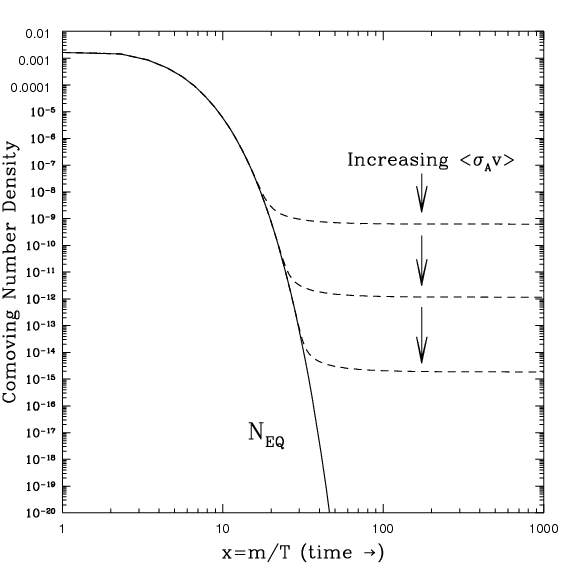
\includegraphics[width=\linewidth]{Documents/Thesis/Figs/Thermal-freeze-out-of-dark-matter-for-different-annihilation-cross-sections-c-Dan.jpg}
    \caption{Freeze-out of dark matter for different annihilation cross-sections. Source: Dan Hooper, [hep-ph] FERMILAB-CONF-09-025-A \cite{hooper2009tasi2008lecturesdark}.}
    \label{fig:freezeout}
\end{wrapfigure}

Fig. \ref{fig:freezeout} is a plot of comoving number density (the number density scaled by the Hubble constant), $Y = \frac{n}{s}$ where $s$ is the entropy density, against inverse temperature of the universe, $x = \frac{m}{T}$, where $m$ is the mass of DM, $T$ being temperature. If DM relic density does not change, it would follow the black solid line. However, that is not the case, as the number density of DM actually follows the dotted line. A higher cross-section means particles stay in equilibrium longer, resulting in a lower relic abundance, and vice versa.

We can derive an expression for $\frac{dY}{dx}$ from Eqn. \ref{eqn:boltzmann}. By using the product rule,we can write the following equation:
\begin{equation}
    \begin{split}
        \frac{d}{dt} \left(\frac{n}{s} \right) =& \frac{s\frac{dn}{dt} - n\frac{ds}{dt}}{s^2}
        \\=& \frac{1}{s}\frac{dn}{dt} - \frac{n}{s}\frac{ds}{dt}
        \\=& \frac{1}{s}\frac{dn}{dt} - \frac{n}{s^2}(-3Hs)
    \end{split}
    \label{eqn:dydt}
\end{equation}

Due to the fact that $sa^3 = \text{constant}$, so $\frac{ds}{dt} = -3Hs$. We can substitude Eqn. \ref{eqn:dydt} and $Y = \frac{n}{s}$ into Eqn. \ref{eqn:boltzmann}:
\begin{equation}
    \begin{split}
        \frac{dY}{dt} &= \frac{1}{s}\left(-3Hn - \braket{\sigma\nu}(n^2 - n^2_{eq})\right) - \frac{n}{s^2}(-3Hs)
        \\&= -s\braket{\sigma\nu}(Y^2 - Y^2_{eq})
    \end{split}
\end{equation}
Considering temperature dependance, we now use the expression $\frac{dT}{dt} = -HT$. This is due to the fact that in the early universe where it was radiation dominated, temperature scaled like $\frac{1}{a}$. Using that information, we can write:
\begin{equation}
    \begin{split}
            T(t) &= \frac{T_0}{a(t)}
            \\ \frac{dT(t)}{dt} &= -T_0\frac{\dot a(t)}{a(t)^2}
            \\ &= -\frac{T_0}{a(t)}\frac{\dot a(t)}{a(t)}
            \\ &= -HT(t)
    \end{split}
\end{equation}

Using another chain rule, it is obvious that:
\begin{equation}
    \frac{dY}{dT} = \frac{dY}{dt}\cdot\frac{dt}{dT} = \frac{s}{HT}\braket{\sigma\nu}(Y^2 - Y^2_{eq})
\end{equation}

In order to reach the final form of the equation, $\frac{dY}{dx}$, we use the chain rule $\frac{dY}{dx} = \frac{dY}{dT}\cdot\frac{dT}{dx}$, where 
\begin{equation}
    \begin{split}
        \frac{d}{dx}\left(\frac{m}{x}\right) &= \frac{x\frac{dm}{dx} - m\frac{dx}{dx}}{x^2} 
        \\ &= -\frac{m}{x^2} \text{ ,}\qquad \text{as }\qquad \frac{dm}{dx}= 0
    \end{split}
\end{equation}
Giving the final equation:
\begin{equation}
        \frac{dY}{dx} = \frac{dY}{dT}\cdot\frac{dT}{dx} = -\frac{s}{HT}\left(-\frac{m}{x^2}\right)\braket{\sigma\nu}(Y^2 - Y^2_{eq})
\end{equation}

\begin{equation}
    \boxed{\text{ }\frac{dY}{dx} = -\frac{s}{Hx}\braket{\sigma\nu}(Y^2 - Y^2_{eq})\text{ }}
    \label{eqn:boltzmann_xy}
\end{equation}

From the Boltzmann equation, one can derive an expression for DM relic density. Knowing the expressions for $s$ and $H$, and from the equation above (Eqn. \ref{eqn:boltzmann_xy}), one has
\begin{equation}
    s = \frac{2 \pi^2}{45}{g_s}T^3, \qquad 
    H = \frac{\pi}{3}\sqrt{\frac{g_*}{10}}\frac{m^2}{x^2 M_{Pl}}
    \label{eqn:s_and_H}
\end{equation}
Substitution of expressions in Eqn. \ref{eqn:s_and_H} into Eqn. \ref{eqn:boltzmann_xy}:
\begin{equation}
    \begin{split}
        \frac{dY}{dx} &= \frac{2\pi^2}{45}\left(\frac{3}{\pi}g_s\sqrt{\frac{10}{g}}\right)\frac{1}{x}\braket{\sigma \nu}(Y_{eq}^2 - Y^2) \\
        &= \frac{1}{x^2}\left(\frac{2 \pi}{15}g_s\sqrt{\frac{10}{g_p}}m_{DM}M_{Pl}\right)\braket{\sigma \nu}(Y_{eq}^2 - Y^2) \\
        \text{setting } \lambda &= \left(\frac{2 \pi}{15}g_s\sqrt{\frac{10}{g_p}}m_{DM}M_{Pl}\right)\braket{\sigma \nu}, \\
        &= \frac{\lambda}{x^2}(Y_{eq}^2 - Y^2)
    \end{split}
\end{equation}

We can solve for x:
\begin{equation}
    \begin{split}
        \frac{dY}{dx} &= \frac{\lambda}{x^2} (Y_{eq}^2 - Y^2)
        \\\int \frac{1}{Y_{eq}^2 - Y^2}\text{ } dY &= \int\frac{\lambda}{x^2}\text{ } dx
        \\ 
    \end{split}
\end{equation}
\section{The Inert Two Higgs Doublet Model (i2HDM)}
\label{sec:i2HDM}
In the i2HDM, we propose two doublets, $\Phi_1$, $\Phi_2$ - where the first doublet is active and second doublet is inert. The latter does not share its degrees of freedom with other particles (or, it does not couple to fermions via Yukawa interactions \cite{Belyaev_2022}), and has no VEV; unlike the former which is just the SM Higgs doublet, which has a VEV. We can invoke a new set of particles arising from $\Phi_2$- $h^\pm, h_1,$ and $h_2$, where $m_{h_1} < m_{h_2}$ and $m_{h_1} < m_{h^\pm}$. The lightest particle, $h_1$ is the DM candidate particle.

As mentioned in the Introduction (Section \ref{sec:introduction}), i2HDM is an extension of SM that introduces new scalar particles that could be candidates for DM.

The field, along with its Hermitian conjugate is:
\begin{align}
    &\Phi_2 = \frac{1}{\sqrt{2}}
        \begin{pmatrix}
            {\sqrt{2}h^+} \\
            {h_1 + ih_2 }
        \end{pmatrix}&
    &\Phi_2^\dagger = \frac{1}{\sqrt{2}} 
        \begin{pmatrix}
            {\sqrt{2}h^-} \\
            {h_1 - ih_2 }
        \end{pmatrix}
\end{align} 

The (scalar) potential is expressed as:
\begin{equation}
    \begin{split}
        V(\Phi_1, \Phi_2) =& -m_1^2(\Phi_1^\dagger\Phi_1) - m_2^2(\Phi_2^\dagger\Phi_2) + \lambda_1(\Phi_1^\dagger\Phi_1)^2 + \lambda_2(\Phi_2^\dagger\Phi_2)^2 \\
        &+ \lambda_3(\Phi_1^\dagger\Phi_1)(\Phi_2^\dagger\Phi_2) + \lambda_4(\Phi_2^\dagger\Phi_1)(\Phi_1^\dagger\Phi_2) + \frac{\lambda_5}{2}[(\Phi_1^\dagger\Phi_2)^2 + (\Phi_2^\dagger\Phi_1)^2]
        \end{split}
        \label{eq:higgs_potential}
\end{equation}
Where:
\begin{itemize}
    \item $\Phi_1$ represents the active doublet
    \item $\Phi_2$ represents the inert doublet
    \item $m_1$ is the term which determines the mass of the Higgs boson and symmetry breaking. The negative sign in the first term of Equation \ref{eq:higgs_potential} makes the first term a potential with negative slope, which introduces spontaneous symmetry breaking and gives the active Higgs doublet the VEV.
    \item $m_2$ is the mass term of the inert Higgs doublet (which helps determine the masses of the extra particles, $h_1$, $h_2$ and $h_\pm$)
    \item $\lambda_{1, 2}$ are self coupling terms of the doublets. $\lambda_1$ determines the mass of the Higgs boson and $\lambda_2$ determine the \todo{determine what?}
    \item $\lambda_{3, 4, 5}$ are the coupling terms of doublet interaction
\end{itemize}
Furthermore, we impose additional parametrisation in terms of mass differences that allow better visualisation of parameter space \cite{Belyaev_2022}, the reason which will be prevalent in the next sections when considering constrains:
\begin{align}
\label{eq:mass_diff_1}
    \Delta m_0 = m_{h_2} - m_{h^\pm},\\ \notag
    \Delta m_1 = m_{h_2} - m_{h_1},\\ \notag
    \Delta m_+ = m_{h^\pm} - m_{h_1}
\end{align}

\subsection{Constraints of the i2HDM}
We have four parameters to scan across: $m_{h_1}$, $\Delta m_0$, $\Delta m_+$, and $\lambda_{345}$ ($\lambda_3 + \lambda_4 + \lambda_5$), with $\lambda_2 = 1$. We can set $\lambda_2 = 1$ because $\lambda_2$ does not affect DM phenomenology at the tree level\footnote{lowest-order approximation in perturbation theory, where Feynman diagrams do not include loops (closed paths)}\cite{Belyaev:2016lok}; it only governs self interaction of the inert Higgs doublet, does not affect physical observables, and the DM candidate $h_1$ is only dependent on $\lambda_3$, $\lambda_4$ and $\lambda_5$ (Equation \ref{eqn:massdmscalar}). 

While $\lambda_2$ does not appear explicitly in the relevant interactions, it indirectly contributes to vacuum stability, ensuring a consistent and physically viable model. Setting $\lambda_2 = 1$ also greatly reduces computing load and time. The masses of $h_2$, $h_\pm$ are then calculated using Eqn. \ref{eq:mass_diff_1}.

This will be a random scan of the parameter space, done with the software \verb|microOMEGAS|, version 6.1.15. Through theory and experiments, there are certain constraints that will have to be applied to the scan such that a proper search can be done.\todo{rewrite this to make this paragraph more clear}

\subsubsection{Constraints from vacuum stability}
First of all, we need to ensure that the potential is bounded from below to ensure stability \cite{Deshpande:1977rw}. This can be done by imposing limits for $\lambda$ couplings:
\begin{equation}
    \begin{split}
    \lambda_1>0,& \qquad
    \lambda_2>0, \qquad
    \lambda_3> -2 \sqrt{ \lambda_1 \lambda_2}, \\
    &\lambda_3 + \lambda_4 - |\lambda_5| > -2 \sqrt{ \lambda_1 \lambda_2}.
    \end{split}
    \label{eq:potential_stability}
\end{equation}
We can describe the parameter space of the i2HDM as \cite{Belyaev:2016lok}:
\begin{equation}
    \begin{split}
        m_{h_1}, \qquad m_{h_2} > m_{h_1}, \qquad m_{h^\pm} > m_{h_1}, \\
        \lambda_2 > 0, \qquad \lambda_{345} > -2\sqrt{\lambda_1 \lambda_2}
    \end{split}
\end{equation}

Where $m_{h_1}$, $m_{h_2}$ and $m_{h^\pm}$ are the masses of the 2 neutral and 2 charged inert scalars. This is to ensure that the Higgs potential is bounded from below and has a neutral, non-charge breaking vacuum, which is only satisfied if:
\begin{equation}
    \lambda_4 - |\lambda_5| < 0
\end{equation}

One could evaluate the masses of these physical scalars \cite{Belyaev:2016lok}:
\begin{align}
    \label{eqn:scalar_equations}
    &m_{Higgs}^2 = 2\lambda_1v^2 = 2m^2_1,\\
    &m_{h_\pm} = \frac{1}{2}\lambda_3v^2-m^2_2 \\
    \label{eqn:massdmscalar}
    &m_{h_1}^2 = \frac{1}{2}(\lambda_3 + \lambda_4 - |\lambda_5|)v^2 - m_2^2\\
    &m_{h_2}^2 = \frac{1}{2}(\lambda_3 + \lambda_4 + |\lambda_5|)v^2 - m_2^2 > m^2_{h_1}
\end{align}

and the mass differences: 
\begin{align}
    &m_{h_2}^2 - m_{h_1}^2 =  |\lambda_5|v^2, \\
    &m_{h_\pm}^2 - m_{h_2}^2 = -\frac{1}{2}(\lambda_4 - |\lambda_5|)v^2
\end{align}

$m_{h_1}$, $m_{h_2}$, $m_{h_\pm}$ and $\lambda_{345}$, along with mass differences $\Delta m_{0, 1, +}$, are parameters of interest of this study. $\lambda_{345}$ is an important parameter as it is involved in the $H\rightarrow h_1,h_1$ and $h_1,h_1 \rightarrow H$ (written in short as $Hh_1h_1$) interaction vertex. $\lambda_1$ is not a free parameter due to the reasons discussed earlier.

In addition to that, we consider constraints due to symmetry breaking. We impose that, from \cite{Belyaev:2016lok, Ginzburg2010}:
\begin{equation}
    m_{h_1}^2 >
        \begin{cases}
         0, & |R| < 1\\
         (R-1) \sqrt{\lambda_1\lambda_2} v^2, & R>1
        \end{cases}
        \label{eqn:R}
\end{equation}

Where:
\begin{equation}
    R = \frac{\lambda_{345}}{2\sqrt{\lambda_1\lambda_2}}
\end{equation}
$\lambda_1$, the self coupling term for the Higgs boson can be evaluated (from Equation \ref{eqn:scalar_equations}):
\begin{equation}
    \begin{split}
        \lambda_1 &= \frac{m^2_{Higgs}}{2 v^2}
                \approx\frac{125^2}{2\cdot 246 ^ 2} \\
                &\approx0.129
    \end{split}
\end{equation}

In addition, we can see Eqn. \ref{eqn:R} can be rewritten as:
\begin{equation}
    \lambda_{345} < 2\left( \frac{m_{h_1}^2}{v^2} + \sqrt{\lambda_1\lambda_2}\right)
\end{equation}
This is another one of our constraints on $\lambda_{345}$.

\subsubsection{Constraints from perturbativity and unitarity}
As shown in \cite{Belyaev:2016lok}, where \cite{Aruhrib2012Inert} was considered, it was shown that $\lambda_{345}$ had to obey these constraints\improvement{add more info, too little!}:
\begin{equation}
    -1.47 < \lambda_{345} < 4\pi
    \label{eqn:l345_pert}
\end{equation}
And $m_{h_1, h_2, h_\pm}$ had to obey:
\begin{equation}
    10\text{ Gev} < m_{h_1, h_2, h_\pm} < 1000\text{ GeV}
    \label{eqn:masses_pert}
\end{equation}

\subsubsection{Constraints from LEP and EWPT (Electroweak Precision Data)}
There is a universal low-mass exclusion where LEP-II searched for pair produced scalars and set the lower mass limits:
\begin{equation}
    \begin{split}
        &m_{h_1} < 45  \text{ GeV}, \qquad m_{h_2} < 45 \text{ GeV}
         \\ &\text{or: } \qquad m_{h_\pm} <70 \text{ GeV}
    \end{split}
    \label{LEP-1}
\end{equation}

LEP has also placed \textbf{kinematic constraints} on the masses of $h_1, h_2$ and  $h_\pm$:
\begin{equation}
    \begin{split}
        &m_{h_1} + m_{h_\pm} > m_{W^\pm}, \qquad m_{h_1} + m_{h_\pm} > m_{Z^0},
        \\&m_{h_2} + m_{h_\pm} > m_{W^\pm}, \qquad 2m_{h_\pm} > m_{Z^0}, 
    \end{split}
\label{LEP-2}
\end{equation}
From \ref{LEP-2}, we can see that the constraints follow the W and Z boson masses. This is because the decay of $Z \rightarrow h_1h_2$ or $W^- \rightarrow h_-h_1$ and others is forbidden, as it would contribute to the invisible decay width of the Z boson which LEP-I has placed tight constraints on (decays such as $Z\rightarrow \nu \bar{\nu}$; the portion of the decay width that cannot be detected directly) as $\Gamma(Z\rightarrow \text{invisible}) = 499.0 \pm 1.5 \text{ MeV}$, where deviation from this means evidence for new invisible particles. If $Z \rightarrow h_1h_2$ was allowed, and $ h_1,h_2$ were stable enough to escape detection, this would cause deviations in the extremely precisely measured invisible width of the Z boson.

From LEP II \cite{Lundstr_m_2009}, there are the additional constraints on the masses and mass differences, due to a visible dijet/dilepton signal. This means that for a certain mass difference ($m_{h_2} - m_{h_1} > 8\text{ GeV}$, given by LEP) one would see a signal i.e.: $e^+e^-$ or $\mu^+ \mu^-$ along with some energy (which corresponds to the DM particles). However LEP-II did not observe such cases, therefore the parameter space is excluded. 

Via LEP-II experiments, we require the following parameter space to be excluded, as they do not generate the signal (note that all the conditions have to be met in order for the point to be excluded):
\begin{equation}
    \begin{split}
        m_{h_1} < 80 &\text{ GeV}, \qquad
        m_{h_2} < 100 \text{ GeV},
        \\
        &m_{h_2} - m_{h_1} > 8\text{ GeV},
    \end{split}
\label{LEP-3}
\end{equation}
These regions, often referred to as "LEP holes", represent parts of parameter space where the production cross section or decay kinematics result in events that are either undetectable or mimic SM backgrounds closely. Thus, although the masses are small, these points evade exclusion due to limited detection sensitivity. While LEP constraints exclude low-mass and large-splitting scenarios, they are complementary to relic density and direct detection bounds. For example, compressed spectra allowed by LEP may still be ruled out by insufficient annihilation.

From \cite{gfitter2018}, we introduce parameters $S$, $T$ and $U$, the Peskin-Takeuchi parameters \cite{PeskinTakeuchi1990} which describe potential new physics contributions \unsure{what does this even mean}{to electroweak radiative corrections}. For a Higgs boson mass of 125 GeV, the latest values for $S$ and $T$ when setting $U = 0$ are \cite{gfitter2018}:
 \begin{align}
     S|_{U=0} = 0.04 \pm0.08, \qquad
     T|_{U=0} = 0.08\pm0.07
 \end{align}
With a correlation coefficient of $+0.92$. Setting $U = 0$ allows simplification in parameter space, requiring only focus on the $S-T$ plane, which are more dominant. This is is common practice as $U$ is related to the $W$ and $Z$ boson, and will be insignificant unless new physics affects them. Defining:
\begin{align}
    x_1 = \frac{m_{h_1}}{m_{h_\pm}}, \qquad 
    x_2 = \frac{m_{h_2}}{m_{h_\pm}}
\end{align}
As well as:
\begin{align}
    &f_a(x) = -5 +12\log(x), \qquad f_b(x) = 3-4\log(x),
    \\
    &f_c(x,y) = 
    \begin{cases}
        \frac{x+y}{2}-\frac{xy}{x-y}\log{\left(\frac{x}{y}\right)}, & x\neq y\\
        0, & x = y
    \end{cases}
\end{align}

The S and T parameters are given \cite{Belyaev:2016lok} with the equations:
\begin{equation}
           S = \frac{1}{72\pi}\frac{1}{(x^2_2 - x^2_1)^3}[x^6_2f_a(x_2)-x^6_1f_a(x_1)+ 9x_2^2x_1^2(x_2^2f_b(x_2)-x^2_1f_b(x_1)] 
    \label{eqn:S}
\end{equation}
\begin{equation}
        T = \frac{1}{32\pi^2\alpha\nu}[f_c(m^2_{h_\pm},m^2_{h_2})
            + f_c(m^2_{h_\pm},m^2_{h_1}) - f_c(m^2_{h_2},m^2_{h_1})]
    \label{eqn:T}
\end{equation}

Notice that for Eqn. \ref{eqn:S} there is a $\frac{0}{0}$ condition when $m_{h_1} = m_{h_2}$, which leads to instability. This is not required for Eqn. \ref{eqn:T} as the function $f_c(x, y)$ handles the instability. By expressing $S$ as a fraction of 2 functions, $\frac{F(x_1, x_2)}{H(x_1, x_2)}$, and applying L'Hopital's Rule, we require 3rd order derivatives for $F$ and $H$. For the case where $x_1 = x_2$, one obtains the equation (the detailed deriviation will be shown in the \ref{appendix}: 
\begin{equation}
    \begin{split}
        S =& \frac{120 x^3f_a(x) + 90 x^4f_a'(x)+18x^5f''_a(x)+x^6f'''_a(x)}{48x^2} \\&+\frac{9x^2\left(24xf_b(x) + 36x^2f_b'(x)+12x^3f_b''(x) + x^4f_b'''(x)\right)}{48x^2}
        \\ =& \frac{1}{24\pi}\left(-5 + 12\log(x) + 3x - 4x\log(x)\right)
    \end{split}
    \label{eqn:S_hopital}
\end{equation}

\subsubsection{Constraints from DM Direct Detection (DD), CMB, Branching Ratio and LZ 2024}
The constraints applied from DM DD experiments are applied via a p-value. A p-value of 0.1 is used, and values greater than 0.1 are accepted to exclude values given by DD experiments.

There also is the chance that the values obtained could have been excluded by the CMB. Energy injections from WIMP annihilation into Standard Model particles during the recombination era could alter the ionization history; this means recombination is delayed and will change how light travels through the universe, and, consequently, the observed CMB anisotropies, which are temperature fluctuations. To comply with measurements from Planck and other CMB experiments, parameter points are checked to ensure that their annihilation cross sections do not lead to excessive energy injection, which would otherwise distort the CMB power spectrum. 

The upper limit of the branching ratio for the invisible Higgs at 95\% confidence level from the latest ATLAS search is \cite{ATLAS:2022yvh}:
\begin{equation}
    Br(\text{Higgs} \rightarrow \text{invisible}) = 0.145
    \label{eqn:branching_ratio}
\end{equation}

The latest results from LZ (Fig. 5 from \cite{aalbers2024darkmattersearchresults}) is used to find new parameter space in the plane $m_{h1}$ against WIMP SI cross sections, which is how likely a WIMP scatters off a nucleon inside a detector. The cross section scales as $\sigma \propto A^2$, where $A$ is the atomic mass number. heavy nuclei are effective because the scattering amplitude acts coherently across all nucleons. DD experiments are optimised for SI interactions due to the $A^2$.

\subsubsection{Constraints from DM Relic Density}
\label{sec:relic density}
DM relic density is the remaining DM from the Big Bang, and there are multiple experiments (PLANCK, WMAP) that calculate various cosmological parameters, one of them being the DM relic density. We can use this very accurate data to limit our parameter space to make the search for DM simpler. The latest experimental value for DM relic density is  \cite{Planck:2018vyg}:
\begin{equation}
    \Omega ^{PLANCK}_{DM} h^2 = 0.11933 \pm 0.00091
\end{equation}

We set the parameter space for the density of the DM relic to ignore the cases of DM overabundance (where $\Omega h^2 > \Omega^{PLANCK}_{DM_{max}}h^2$). DM overabundance is not considered as it leads to inconsistencies with the observed CMB and its constraints \cite{Croon_2024, Zavala_2010}. DM under-abundance is allowed to allow for possible external sources of DM.

For data interpretation purposes, and since \verb|micrOMEGAS| software calculates relic density via tree-level calculation, the theoretical constraints applied to the density of DM relics will be within $\pm10\%$ of the value of $\Omega ^{PLANCK}_{DM} h^2$.
\begin{equation}
    \begin{split}
        \Omega_{DM} h^2 &= 0.11933 \pm 10\% \\
        &\approx 0.119 \pm 0.012
    \end{split}
    \label{eqn:DM relic density value}
\end{equation}

\section{Scanning of Parameter Space}
\label{sec:results}
\subsection{5-D Random Scan}
\label{5-D scan}
A 5-D scan is done across the parameters stated earlier and by applying "cuts" to the 5-D datasets, we can then narrow the parameter space in our search for the DM particle.
We apply cuts in the following order:
\begin{itemize}
    \item Cut 1 - Constraints from vacuum stability (Eqn. \ref{eqn:R}), pertubativity and unitarity (Eqn. \ref{eqn:l345_pert}, \ref{eqn:masses_pert}) 
    \item Cut 2 - Constraints from LEP (Eqn. \ref{LEP-1}, \ref{LEP-2}, \ref{LEP-3}) 
    \item Cut 3 - Constraints from DM direct detection, 
    \item Cut 4 - Constraints from CMB data
    \item Cut 5 - Constraint from branching ratio \ref{eqn:branching_ratio}.
    \item Cut 6 - Constraints on spin-independent WIMP-nucleon cross section, based on latest 2024 results from LZ \cite{aalbers2024darkmattersearchresults}
    \item Cut 7 - EWPT constraints (Eqn. \ref{eqn:S}, \ref{eqn:T})
    \item Cut 8 - Constraint from the experimental value of DM relic density (Eqn. \ref{eqn:DM relic density value}) - also adding an option for a "strict" bound - a $\pm 10 \%$ bound on the value of relic density.
\end{itemize}
These cuts are strategically applied in this manner to clearly show the effects on the parameter space from each cut.
\subsection{2-D Projection}
\label{sec:2D-proj}
We can first consider the relationship between $m_{h_1}$ and $\lambda_{345}$, shown in Fig. \ref{fig:l345_md1}.  

\begin{figure}[h]
    \centering
    \makebox[\textwidth][c]{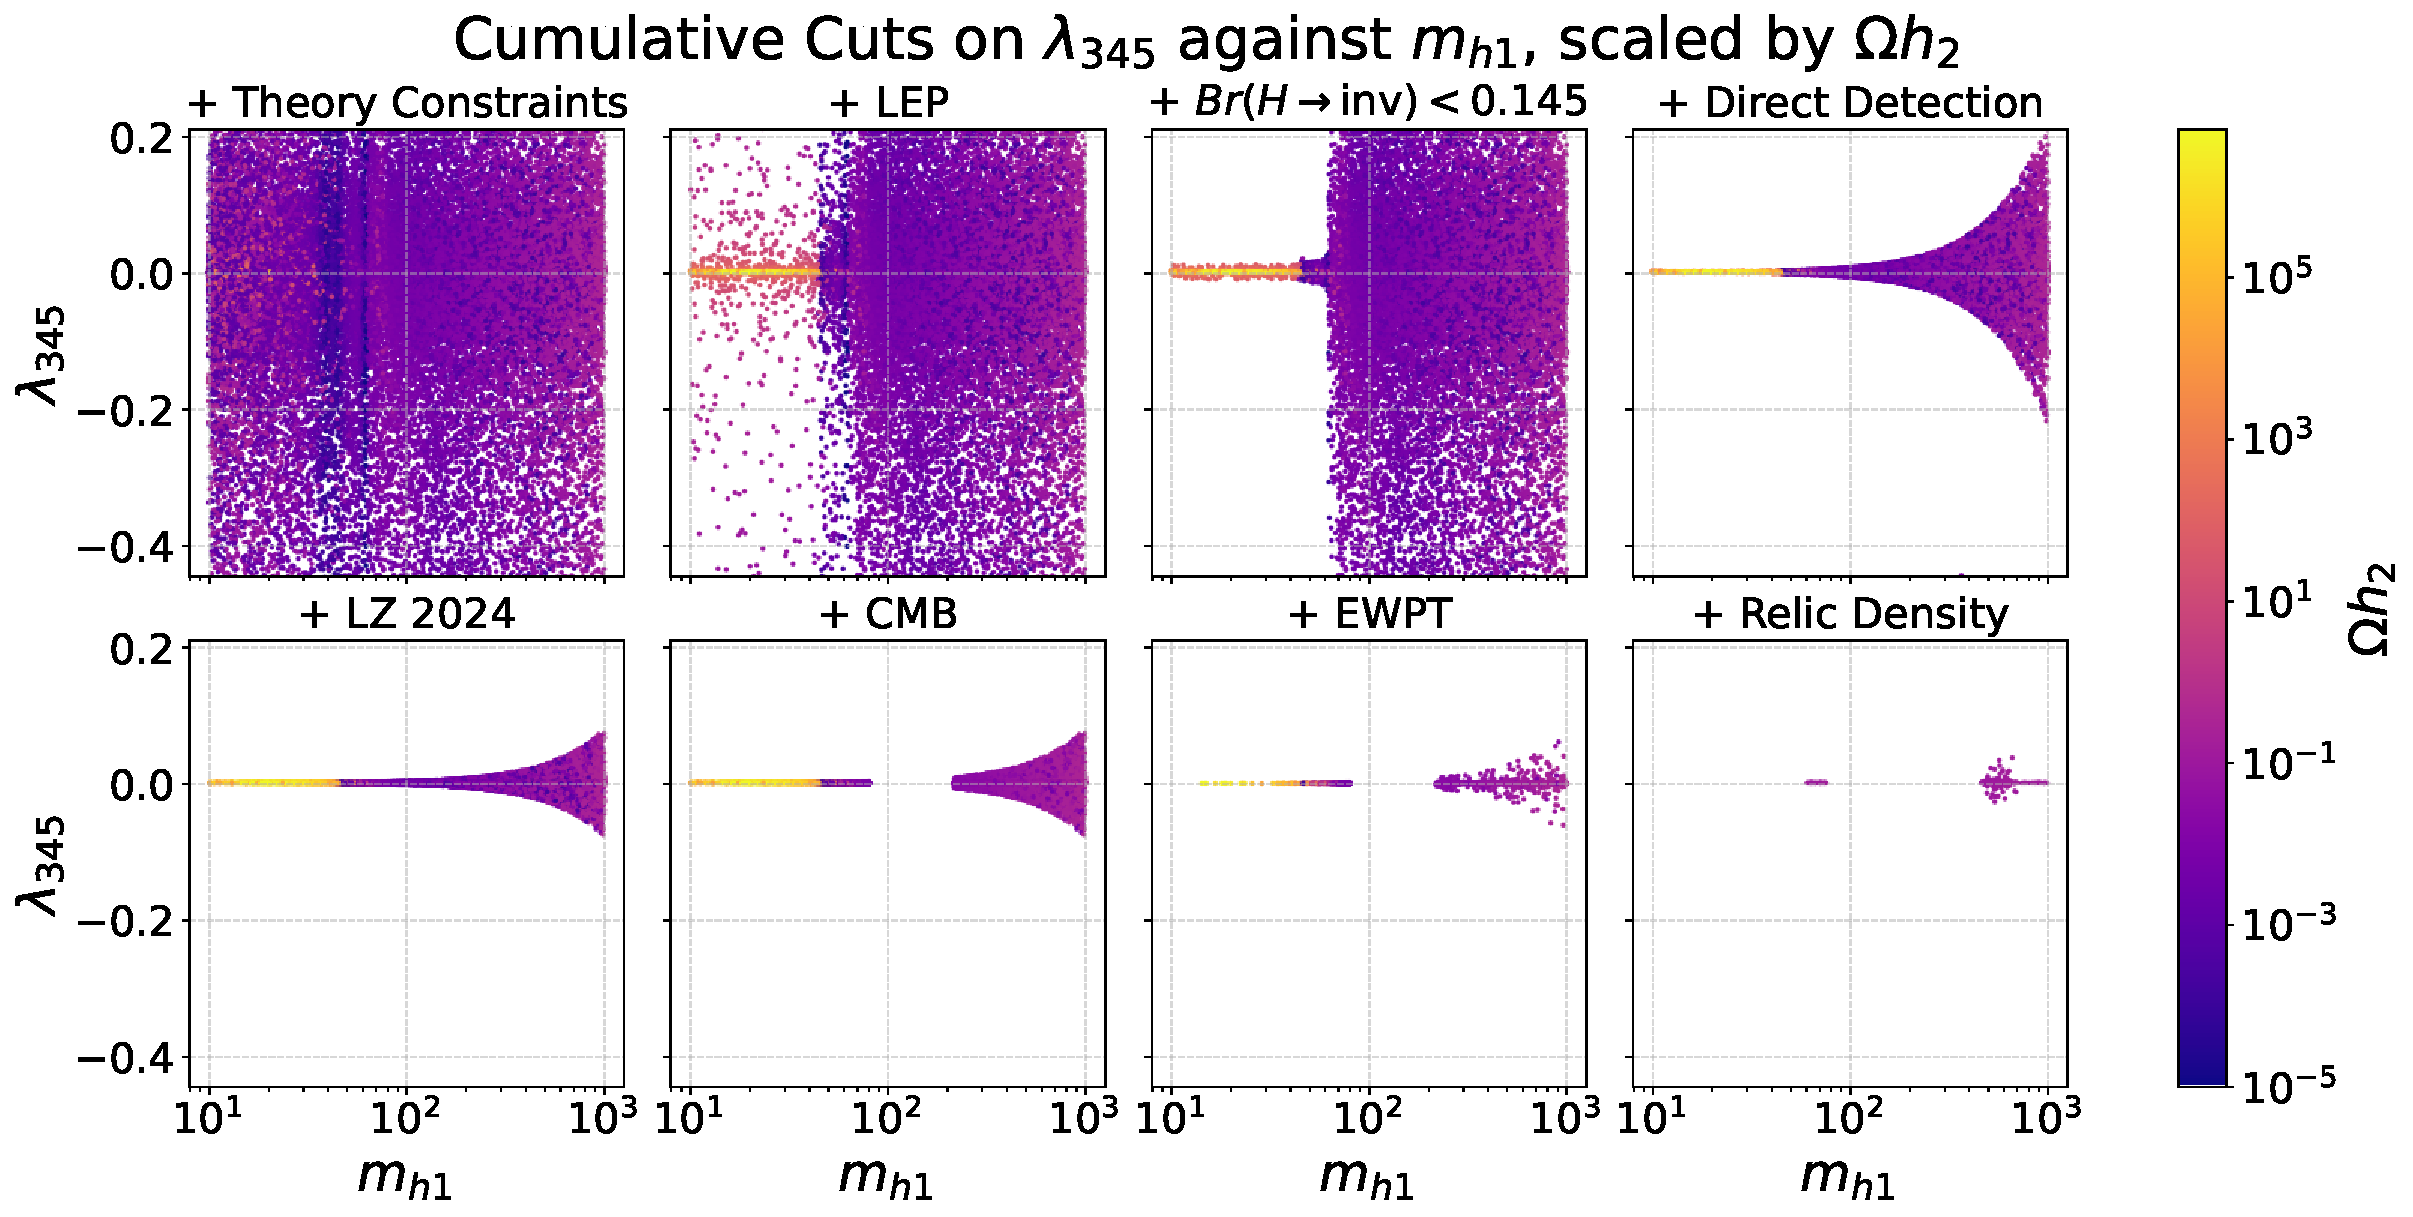
\includegraphics[width=1.2\textwidth]{big_plots_(low_dpi)/l345_against_MD1_Omegah2.pdf}}
    \caption{Plot of $\lambda_{345}$ against $m_{h_1}$, coloured by $\Omega h^2$. From left to right are Cuts 1-8 applied onto the data, with applied plots as their subtitles.}
    \label{fig:l345_md1}
\end{figure}

As the constraints are applied, one can observe 2 regions where $\lambda_{345}$, which is in line with what has been discovered in \cite{Belyaev:2018ext}, which found strong cross section of $100 - 1000 \text{ fb}$. This also gives a good narrowing of the mass of DM particle.

\begin{figure*}[ht]
    \centering
    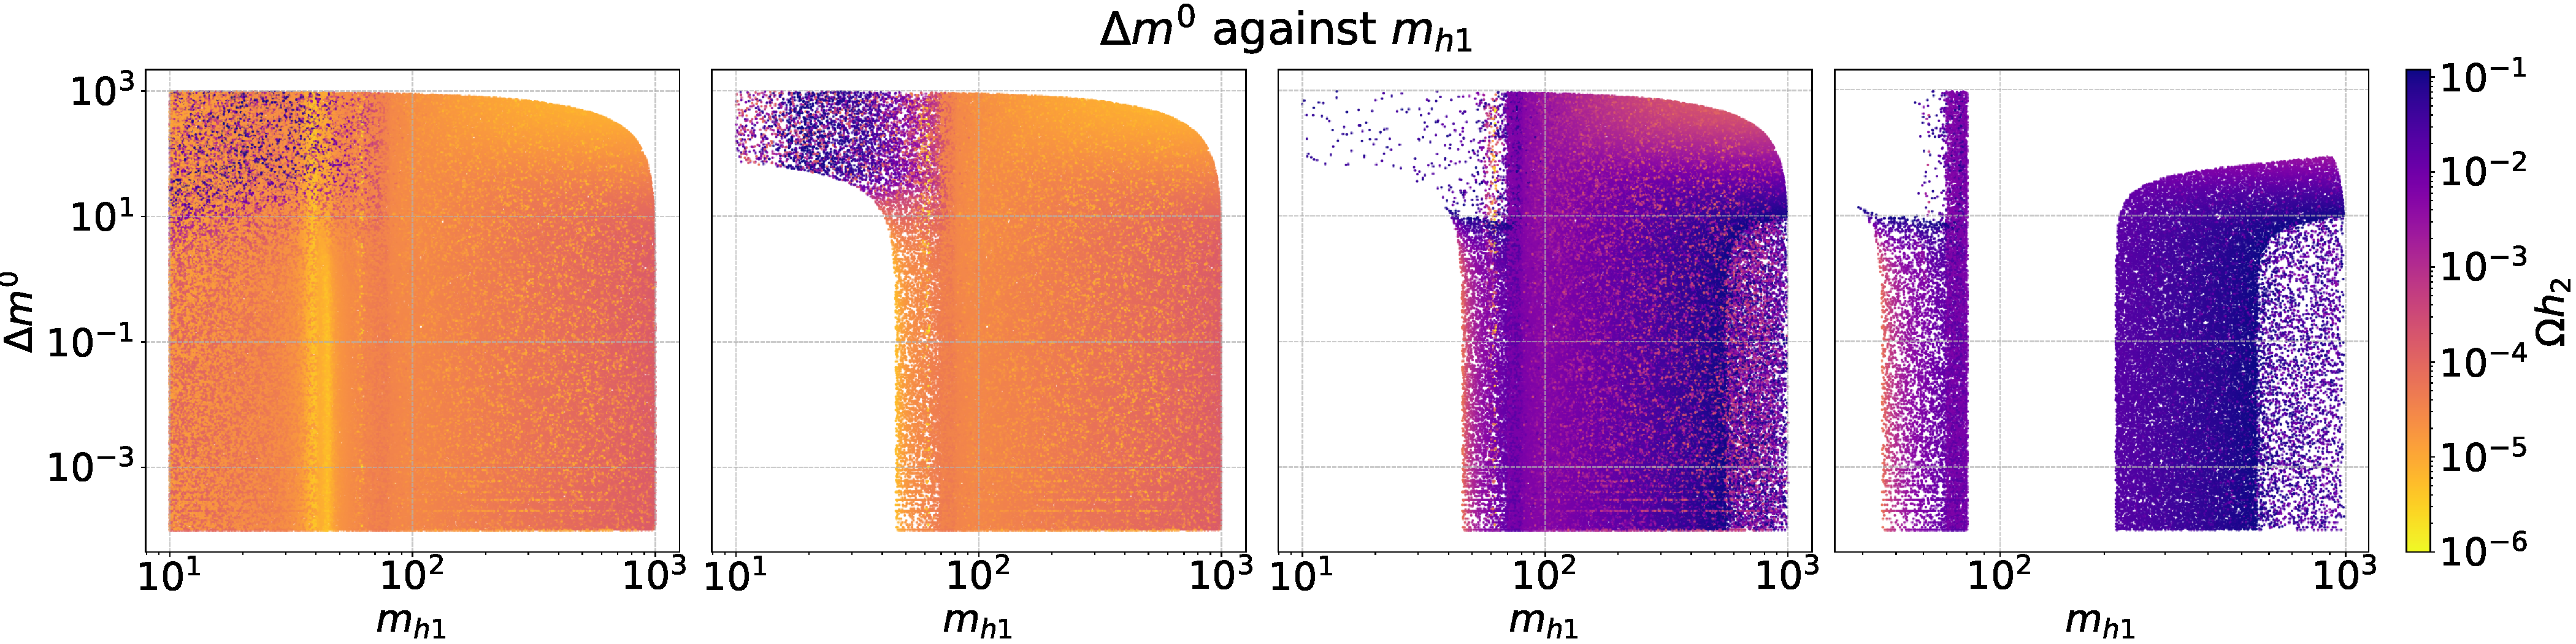
\includegraphics[width=\linewidth]{4plot/DM2_MD1.pdf}
    \caption{Plot of $\Delta m_0$ against $m_{h_1}$, coloured by $\Omega h^2$. From left to right are Cuts 1-8 applied sequentially onto the data.}
    \label{fig:DM2_md1_main}
\end{figure*}

In Fig. \ref{fig:DM2_md1_main}, one can observe the effects of the contraints slowly shrinking the parameter space. The

\subsection{1-D Analysis}
\label{1-D scan}
We can investigate the affect of $\lambda_{345}$ on $\Omega h^2$ (Fig. \ref{fig:MD1_l345_1}, \ref{fig:MD1_l345_100}) as done in \cite{Belyaev:2016lok}:
\begin{figure}[h]
    \centering
    \begin{subfigure}[b]{0.49\textwidth}
        \centering
        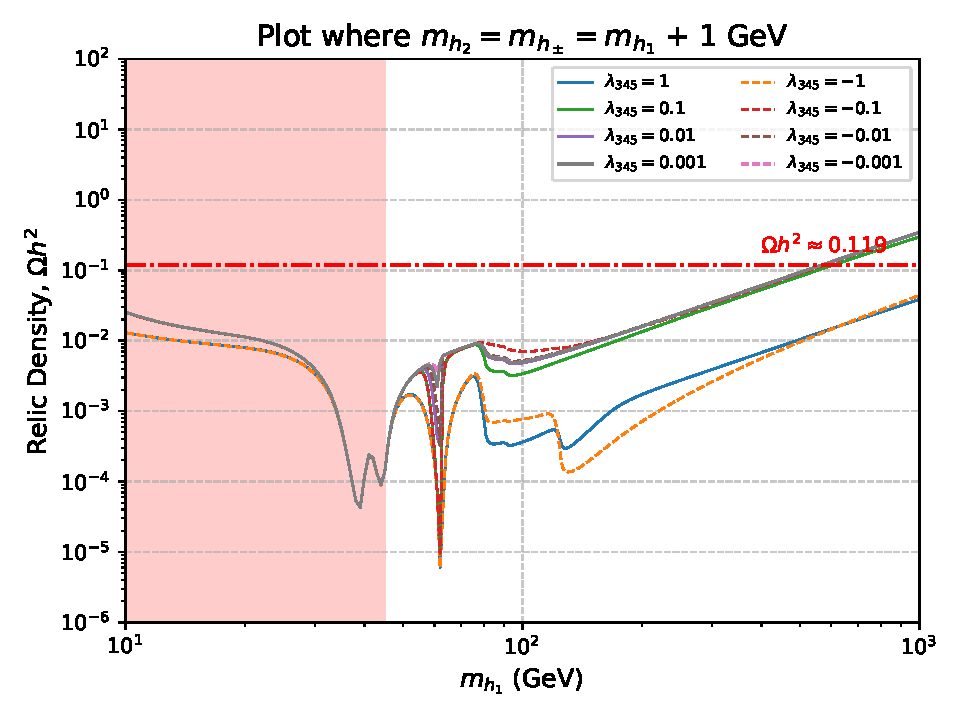
\includegraphics[width=\textwidth]{plots/plot_MD1_l345+1.pdf}
        \caption{Relic density against $m_{h_1}$, the case where $\Delta m_0 = 1$ GeV.}
        \label{fig:MD1_l345_1}
    \end{subfigure}
    \hfill
    \begin{subfigure}[b]{0.49\textwidth}
        \centering
        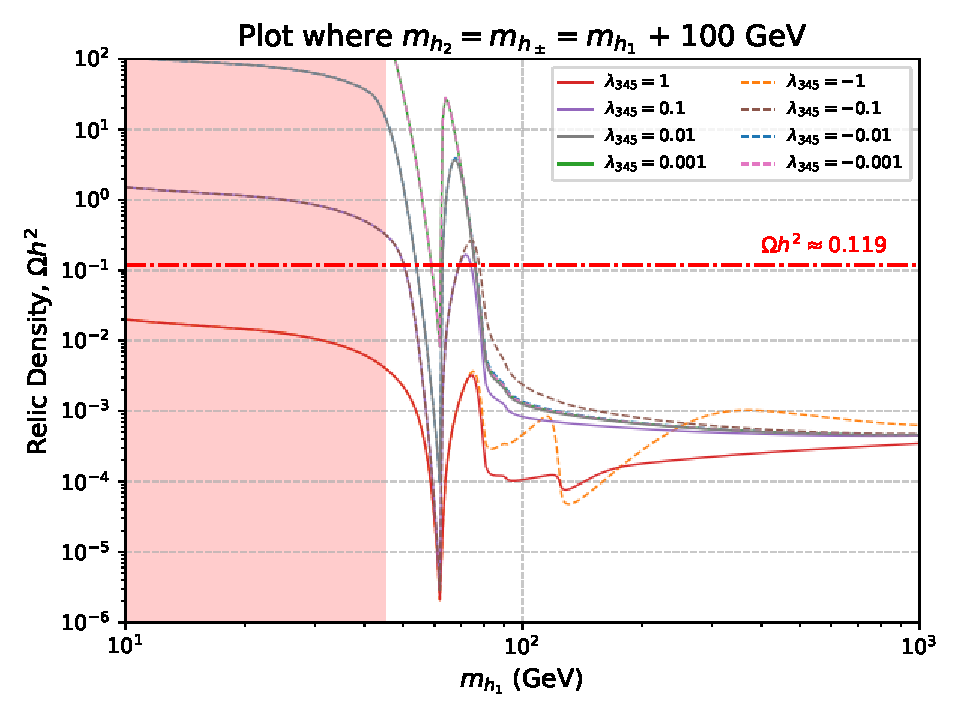
\includegraphics[width=\textwidth]{plots/plot_MD1_l345+100.pdf}
        \caption{Relic density against $m_{h_1}$, the case where $\Delta m_0 = 100$ GeV.}
        \label{fig:MD1_l345_100}
    \end{subfigure}
    \caption{Plots of relic density against $m_{h_1}$ for different mass differences (while keeping $m_{h_1}$ lightest). The red shaded region is the area excluded by LEP, and the red line the upper limit of DM relic density (Eqn. \ref{eqn:DM relic density value}).}
\end{figure}

In Fig. \ref{fig:MD1_l345_1} and \ref{fig:MD1_l345_100}, we alter the masses of the DM candidate, $h_1$ and its complementary particles ($h_2$ and $h_{\pm}$) to observe the relic density, we make a few observations:
\begin{itemize}
    \item The slight dips at 40 and 45 GeV for all values of $\lambda$ is the decay channel where $h_1, h_2 \rightarrow Z^0$ boson, and also the reaction for $h_1, h_{\pm} \rightarrow W_\pm$. The $Z^0$ and $W^\pm$ boson have masses $\sim$80 GeV and $\sim$85 GeV respectively.
    \item At $\sim$60 GeV, there is a dip for all values of $\lambda$ - this is because that is the $h_1,h_1\rightarrow H$ process - the DM DM decay process. 
    \item At 80-90 GeV, we can observe a slight dip for relic density for all values of $\lambda$ except for $\lambda = \pm1$. The reason this happens is because that is the annihilation channel for $h, h \rightarrow Z^0Z^0$ and $h, h \rightarrow W_+ W_-$.
    \item At $\sim$120 GeV, there is no obvious change in relic density except for $\lambda = \pm1$. This is the $h_1,h_1\rightarrow H H$ annihilation channel, which takes place only for big values of $\lambda_{345}$ due to stronger coupling term.
\end{itemize}

\section{2 Lepton Final States at the Collider Level}
We can now calculate the branching ratios for DM decay at the collider level, starting from 2 quarks. The goal here is to be able to find new limits at the 95\% confidence level. Using \verb|CalcHEP|'s \verb|getBr| function, it is easy to obtain the branching ratios. 
\begin{figure}[h]
    \centering
    \begin{subfigure}[b]{0.49\textwidth}
        \centering
        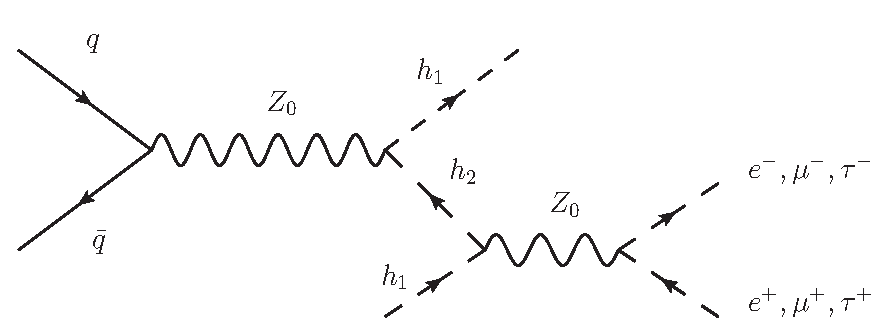
\includegraphics[width=\textwidth]{Feynmann_Diagrams/pp-h1h2.pdf}
        \caption{Production of 2 lepton final states, through decay of the $h_1$ particle to $e^+$ and $e^-$ via the $Z^0$ boson.}
        \label{fig:decay_h2}
    \end{subfigure}
    \hfill
    \begin{subfigure}[b]{0.49\textwidth}
        \centering
        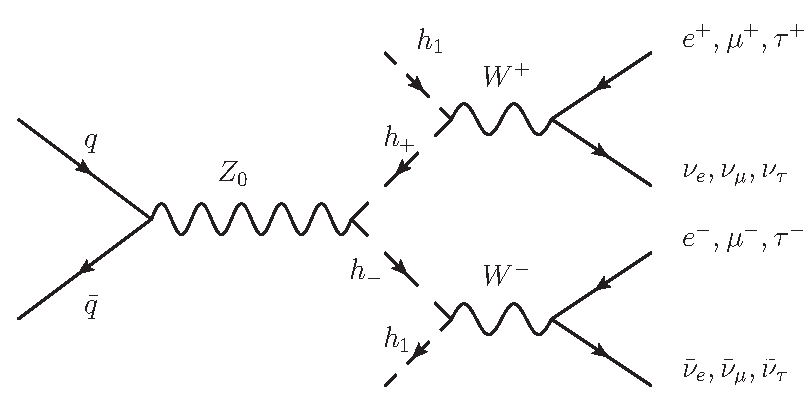
\includegraphics[width=\textwidth]{Feynmann_Diagrams/pp-h+h-.pdf}
        \caption{Production of 2 lepton final states, through decay of the $h_+$ particle to $e^+$ and $\nu_e$ via the $W^+$ boson, and $h_-$ particle to $e^-$ and $\bar{\nu}_e$ via the $W^-$ boson}
        \label{fig:decay_h+}
    \end{subfigure}
    \caption{Feynman diagrams of possible paths for production of 2 lepton final states.}
\end{figure}

For example, we consider the process $p\bar{p} \rightarrow h_1h_2$ where $ h_2\rightarrow h_1 e^+e$ via the $Z$ boson (see Fig. \ref{fig:decay_h2}). The branching ratio of the process is calculated like:
\begin{equation}
    \begin{split}
        Br(h_2 \rightarrow h_1 e^+e) = Br(h_2\rightarrow h_1Z) \times Br(Z\rightarrow e^+e) + Br(h_2 \rightarrow h_1 e^+e)_{non-resonant}
        \label{eqn:branching_Z}
    \end{split}
\end{equation}
where \( Br(h_2 \rightarrow h_1 Z) \) is the branching ratio for the decay of \( h_2 \) into \( h_1 \) and a \( Z \)-boson, and \( Br(Z \rightarrow e^+ e^-) \) is the branching ratio for the \( Z \)-boson decaying into an electron-positron pair. The reason for the additional "non-resonant" summation term is due to the nature of \verb|CalcHEP|, as it calculates a $1\rightarrow2$ decay first, and if that process is has branching ratio of $0$, then it will calculate the contribution from a $1\rightarrow3$ decay.  This  $1\rightarrow3$ decay is known as a "non-resonant 3-body decay", via the $Z^*$ boson, which is a virtual $Z$ boson. Some processes have non-zero $1\rightarrow2$ decays, so just calculating $1\rightarrow3$ decays (directly computing $Br(h_2 \rightarrow h_1 e^+e)$) is going to result in zeros \footnote{There will be no double counting, because if a $1\rightarrow2$ decay path is not possible then the value of the intermediary $Br(Z\rightarrow e^+e)$ will be $0$, giving only $Br(h_2 \rightarrow h_1 e^+e)_{non-resonant}$, the $1\rightarrow3$ decay.}. Likewise, another possible 2 lepton final state can occur through the $W$ boson, for example:
\begin{equation}
    Br(h_-\rightarrow h_1e^- \bar{\nu}_e) = Br(h_-\rightarrow h_1 W^-) \times Br(W^- \rightarrow e^- \bar{\nu}_e) + Br(h_-\rightarrow h_1e^- \bar{\nu}_e)_{non-resonant}
\end{equation}
Here there is a non-resonant 3-body decay via an off-shell ${W^-}$ boson. This is also true for the case of the $W^+$ boson (see Fig. \ref{fig:decay_h+}):
\begin{equation}
    Br(h_+\rightarrow h_1e^+ \nu_e) = Br(h_+\rightarrow h_1 W^+) \times Br(W^+ \rightarrow e^+ \nu_e) + Br(h_+\rightarrow h_1e^+ \nu_e)_{non-resonant}
\end{equation}

By performing a random scan across parameters $\Delta m_3 = m_{h_2} - m_{h_\pm})$ and $\Delta m_+ = m_{h_\pm} - m_{h_1}$ For the decay in Eqn. \ref{eqn:branching_Z}, we can investigate what mass differences have upon the branching ratios.

\begin{figure}[h]
    \centering
    \begin{subfigure}[b]{0.49\textwidth}
        \centering
        \includegraphics[width=\textwidth]{branching_ratio_plots/MD1_100GeV/Brh2ee}
        \caption{Relic density against $m_{h_1}$, the case where $\Delta m_0 = 1$ GeV.}
        \label{fig:Br(h2W+eeh1)}
    \end{subfigure}
    \hfill
    \begin{subfigure}[b]{0.49\textwidth}
        \centering
        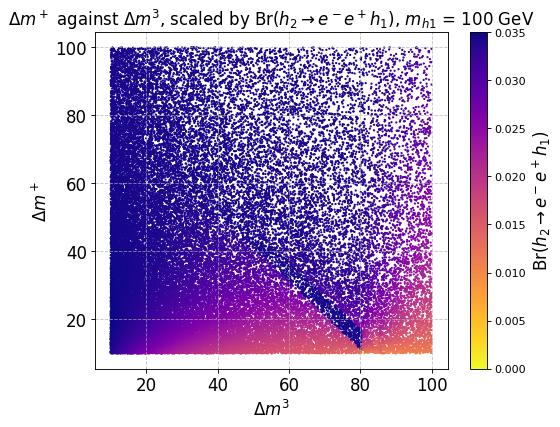
\includegraphics[width=\textwidth]{branching_ratio_plots/MD1_100GeV/__Delta_m_____Delta_m_3__scale_Br__h_2__rightarrow_e_-_e___h_1___MD1_100GeV.jpg}
        \caption{Relic density against $m_{h_1}$, the case where $\Delta m_0 = 100$ GeV.}
        \label{fig:Br(h2W-eeh1)}
    \end{subfigure}
    \caption{Branching ratios of the process }
\end{figure}


From Fig. \ref{fig:Br(h2->e+e-h1),DM2}, one can draw the following conclusions:
\begin{itemize}
    \item At $\Delta m_+= 20\text{ GeV}$ , we can see the branching ratio increase as the value of $\Delta m_3$ decreases. When $\Delta m_3 \approx 90 \text{ GeV}$, there is a low branching ratio of $\approx 1\%$. This is because the decay happens via ${Z}^*$, off mass shell $Z^0$ boson, but at the same time there is another decay route via off mass shell $W^-$ boson, decaying via $h_2 \rightarrow {W^-}^*h_+$. This is due to the fact that:
    \begin{equation}
        \begin{split}
            \Delta m_+ = m_{h_\pm} &- m_{h_1}
            \\ \text{for }\Delta m_+ \approx 0: m_{h_\pm} &= m_{h_1}
            \\ \implies \Delta m_3 + m_{h_2} &= m_{h_\pm}
            \\\implies m_{h_2} >> m_{h_\pm} &= m_{h_1}
        \end{split}
    \end{equation}
    This allows the $h_2$ particle more decay channels, $h_2 \rightarrow {W^-}^*h_+$ being one of them.
    \item At $\Delta m_+= \Delta m_3=80 \text{ GeV}$ (high value), we get branching ratio of $\approx 3\%$. Although one might argue the fact that this means a bigger difference between $m_{h_2}$ and $m_{h_1}$, leading to more decay channels therefore the branching ratio should be low. This is not true in this case as the decay occurs through on mass shell $Z^0$ boson, which is a $1\rightarrow2$ decay, therefore all $1\rightarrow3$ decays are suppressed.
    \item At point $\Delta m_+=\Delta m_3=10 \text{ GeV}$ (low value), comparing both $h_2 \rightarrow e^+ e^- h_1$ and $h_2 \rightarrow e^- \bar{\nu}_e h_+$, which is also another possible decay route (via off mass shell $W^-$). However, $Z^0$ boson will be less off mass shell than the $W^-$ boson; due to $m_{h_2} - m_{h_1} = 20 \text{ GeV}$ and $\Delta m_3= 10 \text{ GeV}$, one can see that $h_2 \rightarrow e^- \bar{\nu}_e h_+$ will be more suppressed, leaving $h_2 \rightarrow e^+ e^- h_1$ the dominant one with branching ratio of $\approx 3.3\%$
    \item One also will notice a dark band at $Br(h_2 \rightarrow h_1 e^+e) \approx 0.033$. One of the points that this is possible is at $\Delta m_+= 20$ and $\Delta m_3=72 \text{ GeV}$. At this point, the value of $m_{h_2} - m_{h_1}$ is $ 92 \text{ GeV}$, which is the mass of the $Z^0$ boson. This enables an on-shell $Z^0$-mediated decay, which maximises the branching ratio into $e^+ e^- h_1$ final state.
\end{itemize}

\subsection{Exclusion Rate}
From \cite{Aruhrib2012Inert}, the exclusion rate $r$ is defined as:
\begin{equation}
    r = \frac{\sigma_{DM}}{\sigma_{95}}
\end{equation}
Where $\sigma_{DM}$ and $\sigma_{95}$ are the cross sections for DM production and the limit of the cross section at $95\%$ confidence level. This equation can be scaled due to the fact that collider luminosity is constantly improving. In the LHC, luminosity depends on the beam parameters: the revolution frequency, number of particles per "bunch" (group of particles) in the beam, and the cross sectional area of the beams at collision point. One can scale $r$ in the following manner;
Signal significance, the measure of how a potential signal stands out from background noise, is expressed as:
\begin{equation}
    \alpha = \frac{S}{\sqrt{B}}
\end{equation}
Where $S$ is the number of potential signals and $B$ the number of background signals. The signal and background can be expressed as $\sigma \mathcal{L}$
\begin{equation}
    \begin{split}
        \alpha &= \frac{\sigma_{signal} \mathcal{L}}{\sqrt{\sigma_{background }\mathcal{L}}}
        \\&= \frac{\sigma_{signal}}{\sqrt{\sigma_{background}}} \sqrt{\mathcal{L}}
        \\&\implies \alpha \sqrt{\sigma_{background}} = \sigma_{limit}^{new}\sqrt{\mathcal{L}}
        \\\sigma_{limit} &=\frac{\alpha \sqrt{\sigma_{background}}}{\sqrt{\mathcal{L}}}  
        \\
    \end{split}
\end{equation}
Keeping $\alpha$ the same, one can derive a relationship for the new limit, $\sigma_{limit}^{new}$ when there is new collider luminosity $\mathcal{L}^{new}$. Since $\sigma_{background}$ is the same for both, and writing the old integrated luminosity as $\mathcal{L}_0$ 
\begin{equation}
    \begin{split}
    \sigma_{limit}^{new} \sqrt{\mathcal{L}^{new}} &= \sigma_{limit}\sqrt{\mathcal{L}_0}
        \\ \sigma_{limit}^{new}&= \sigma_{limit}\sqrt{\frac{\mathcal{L}_0}{\mathcal{L}^{new}}}
    \end{split}
\end{equation}

\section{Conclusion}
\label{sec:conclusion}

\onecolumn
\newpage
\bibliographystyle{unsrt}
\bibliography{references}

\appendix
\section{Deriviation of Equations}
\subsection{Eqn. \ref{eqn:S_hopital}}
\end{document}